\documentclass[11pt,a4paper]{article}
\usepackage{graphicx}
\usepackage{isabelle,amssymb,isabellesym}
\usepackage{pdfsetup}\urlstyle{rm}

%table of contents is too crowded!
\usepackage{tocloft}
\addtolength\cftsubsecnumwidth {0.5em}
\addtolength\cftsubsubsecnumwidth {1.0em}

\begin{document}

\title{The Constructible Universe\\ and the\\
       Relative Consistency of the Axiom of Choice}
\author{Lawrence C Paulson}
\maketitle

\begin{abstract}
  G\"odel's proof of the relative consistency of the axiom of
  choice~\cite{goedel40} is one of the most important results in the
  foundations of mathematics. It bears on Hilbert's first problem, namely the
  continuum hypothesis, and indeed G\"odel also proved the relative
  consistency of the continuum hypothesis. Just as important, G\"odel's proof
  introduced the \emph{inner model} method of proving relative consistency,
  and it introduced the concept of \emph{constructible
    set}. Kunen~\cite{kunen80} gives an excellent description of this body of
  work.
  
  This Isabelle/ZF formalization demonstrates G\"odel's claim that his proof
  can be undertaken without using metamathematical arguments, for example
  arguments based on the general syntactic structure of a formula. Isabelle's
  automation replaces the metamathematics, although it does not eliminate the
  requirement at least to state many tedious results that would otherwise be
  unnecessary.
  
  This formalization~\cite{paulson-consistency} is by far the deepest result
  in set theory proved in any automated theorem prover. It rests on a previous
  formal development of the reflection theorem~\cite{paulson-reflection}.
\end{abstract}

\tableofcontents

\begin{center}
  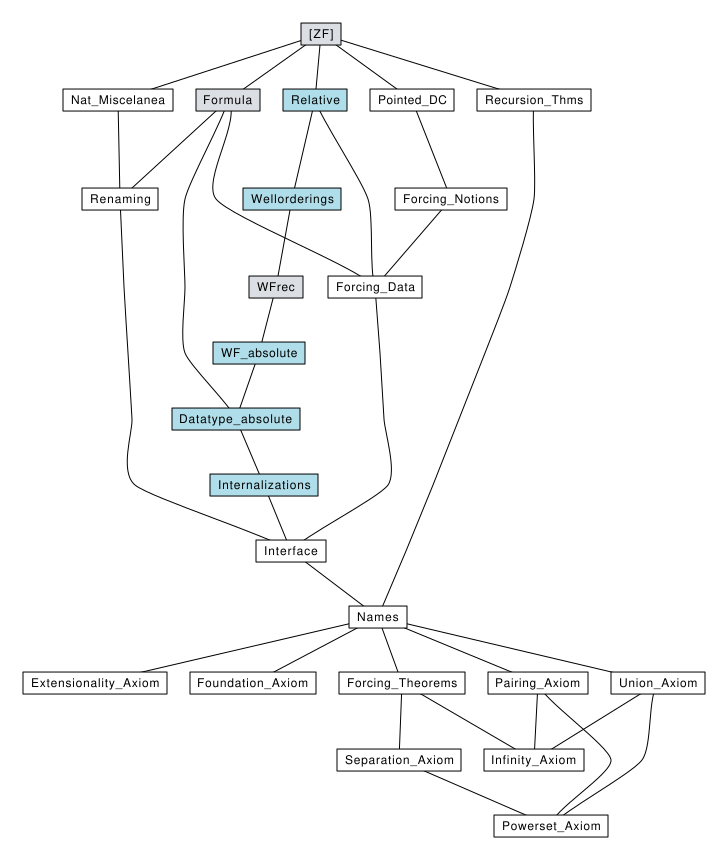
\includegraphics[scale=0.7]{session_graph}
\end{center}

\newpage

\parindent 0pt\parskip 0.5ex

\input{session}

\bibliographystyle{plain}
\bibliography{root}

\end{document}
